% Ubah judul dan label berikut sesuai dengan yang diinginkan.
\section{Desain dan Implementasi}
\label{sec:desaindanimplementasi}

\begin{figure}[ht]
  \centering

  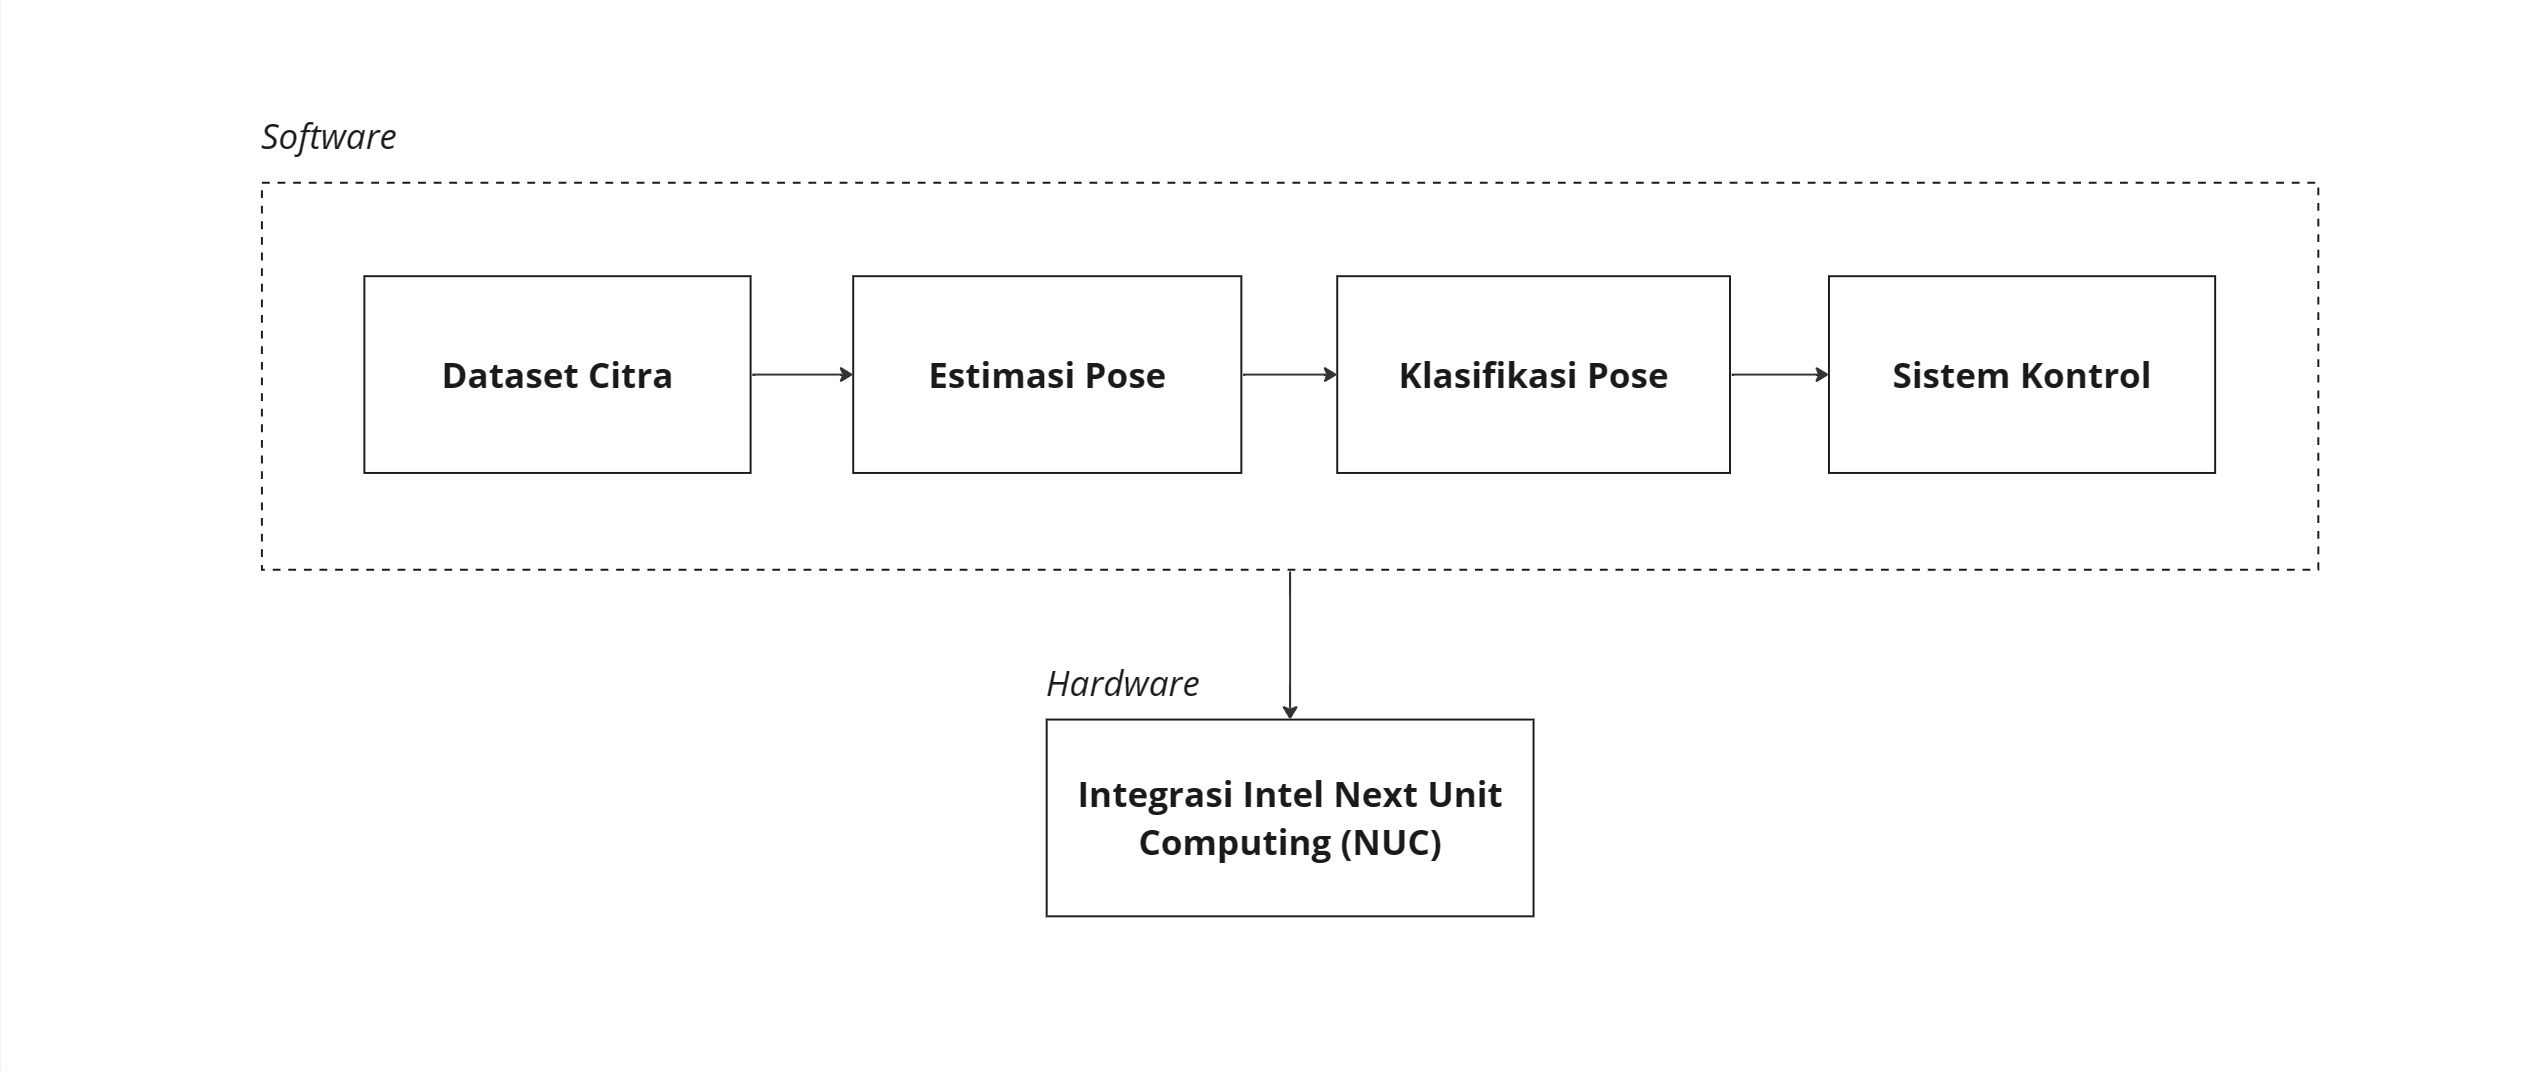
\includegraphics[scale=0.095]{gambar/bab3-block-diagram-nuc.jpg}

  \caption{Alur penelitian}
  \label{fig:blockdiagrammethod}
\end{figure}

\subsection{Dataset Citra}
\label{subsec:datasetcitra}

Dataset yang akan digunakan adalah kumpulan citra berukuran 640 pixel x 480 pixel. Data citra didapatkan dengan bantuan \emph{library} OpenCV untuk mengambil video dengan yang kemudian diekstrak menjadi 30 \emph{frame} untuk setiap data. Adapun digunakan 6 kosakata isyarat BISINDO dengan konteks kosakata umum dan 3 isyarat kontrol untuk memudahkan penggunaan sistem. Secara berurutan, kosakata kontrol "standby" (menandakan transisi kosakata), "\emph{delete}" (menghapus kosakata), dan "\emph{translate}" (konversi ke suara).

\begin{table}[H]
  \caption{Kosakata BISINDO dan Kontrol}
  \label{tb:kosakataBISINDO}
  \centering
  \begin{tabular}{lll}
    \toprule
    \textbf{Kelas} & \textbf{Jumlah Data} & \textbf{Jumlah \emph{Frame}} \\
    \midrule
    Maaf                        & 30            & 30 \\
    Tolong                      & 30            & 30 \\
    Saya                        & 30            & 30 \\
    Nama                        & 30            & 30 \\
    Rumah                       & 30            & 30 \\
    Siapa                       & 30            & 30 \\
    \textit{Standby}                       & 30             & 30 \\
    \textit{Translate}                     & 30             & 30 \\
    \textit{Delete}                        & 30             & 30 \\
    \bottomrule
  \end{tabular}
\end{table}


\subsection{Estimasi Pose}
\label{subsec:estimasipose}

\begin{figure}[ht]
  \centering

  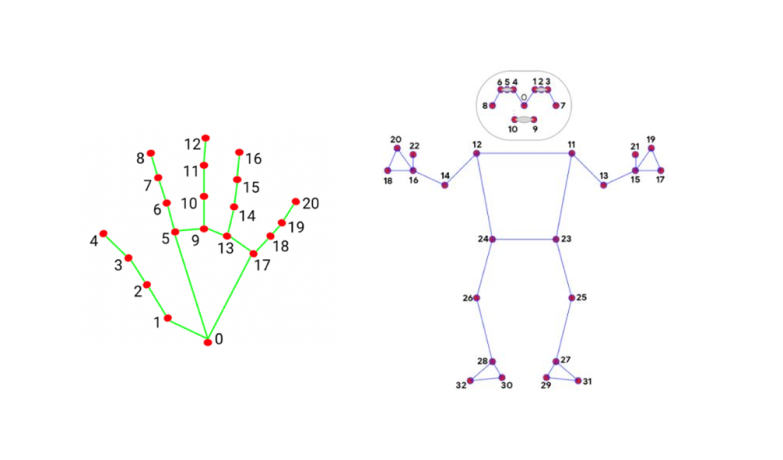
\includegraphics[scale=0.3]{gambar/bab3-pose-combine.png}

  \caption{Mediapipe Pose dan \emph{Hand}}
  \label{fig:estimasipose}
\end{figure}

Untuk setiap citra pada 30 data yang telah dilakukan estimasi pose dengan bantuan \textit{framework} MediaPipe. Dalam pembentukan isyarat BISINDO, bagian tubuh yang bergerak adalah bagian tangan dan lengan. Melalui MediaPipe hand akan dilakukan ekstraksi untuk 21 \textit{landmark} pada bagian tangan, sehingga total \textit{landmark} untuk tangan kanan dan kiri adalah 42 \textit{landmark}. Pada MediaPipe pose akan dilakukan ekstraksi pada bagian bahu sampai lengan sehingga \textit{landmark} yang akan digunakan hanya pada posisi 11 hingga 22 sehingga total \textit{landmark} untuk bagian tubuh adalah 12 \textit{landmark}. Untuk setiap \textit{landmark} yang didapatkan data koordinat x dan y. Data ini kemudian dilakukan normalisasi untuk menghasilkan model yang \textit{scale invariant} (adaptasi terhadap bentuk pengguna) dan \textit{position invariant} (adaptasi terhadap posisi pengguna). Adapun berikut adalah rumus normalisasi yang akan digunakan:

\begin{equation}
  \label{eq:shouderWidthNorm}
  w = \sqrt{(x_{ka} - x_{ki})^2 + (y_{ka} - y_{ki})^2}
\end{equation}

\begin{equation}
  \label{eq:shoulderMidpointNorm}
  x_m = \frac{x_{ka} + x_{ki}}{2} ; \\
   y_m = \frac{y_{ka} + y_{ki}}{2}
\end{equation}

\begin{equation}
  \label{eq:normalization}
  x'_i = \frac{x_i - x_m}{w} ;  \\
   y'_i = \frac{y_i - y_m}{w}
\end{equation}

\subsection{Klasifikasi Pose}
\label{subsec:klasifikasipose}

Model LSTM yang digunakan memiliki arsitektur sekuensial untuk menggabungkan serangkaian layer demi menghasilkan model penerjemah bahasa isyarat yang berperforma baik. Layer pertama adalah TimeDistributed dengan Dense layer berjumlah 128 unit, aktivasi 'tanh', dan input berbentuk (30, 108), di mana setiap frame diproses secara independen dengan konsistensi Dense layer untuk setiap frame. Layer kedua adalah LSTM pertama dengan 128 unit, return\_sequences=True, aktivasi 'tanh', dan input berbentuk (30, 108). Layer ketiga adalah Dropout layer dengan nilai 0,5 untuk mencegah weight yang terlalu tinggi. Layer keempat adalah LSTM kedua dengan 128 unit, return\_sequences=False, dan aktivasi 'tanh', diikuti Dropout layer dengan nilai 0,5. Untuk menyederhanakan kompleksitas data keluaran dari dua LSTM layer, digunakan Dense layer dengan 128 unit dan aktivasi 'relu', diikuti Dropout layer dengan nilai 0,2 untuk mencegah overfitting. Layer terakhir adalah Dense layer dengan aktivasi 'softmax' dan jumlah unit sesuai dengan jumlah kategori. Model ini dikompilasi menggunakan optimizer Adam dan categorical crossentropy sebagai fungsi loss, dengan metrik akurasi kategorikal untuk memantau performa selama pelatihan.

\subsection{Sistem Kontrol}
\label{subsec:sisitemkontrol}
Sistem kontrol adalah serangkaian proses yang akan mengatur bagaimana nantinya bahasa isyarat akan dideteksi, melakukan penanggulangan terhadap adanya kesalahan pendeteksian, menyatukan berbagai kata dalam bentuk kalimat, penghapusan kosakata, dan penerjemahan kalimat dalam bentuk suara. Penggunaan sistem kontrol ini diharapkan akan memudahkan pengguna dalam menggunakan sistem penerjemah. Sistem kontrol akan dibagi menjadi 2, yaitu program deteksi bahasa isyarat dan program pembentukan kalimat.

\begin{figure}[H]
  \centering

  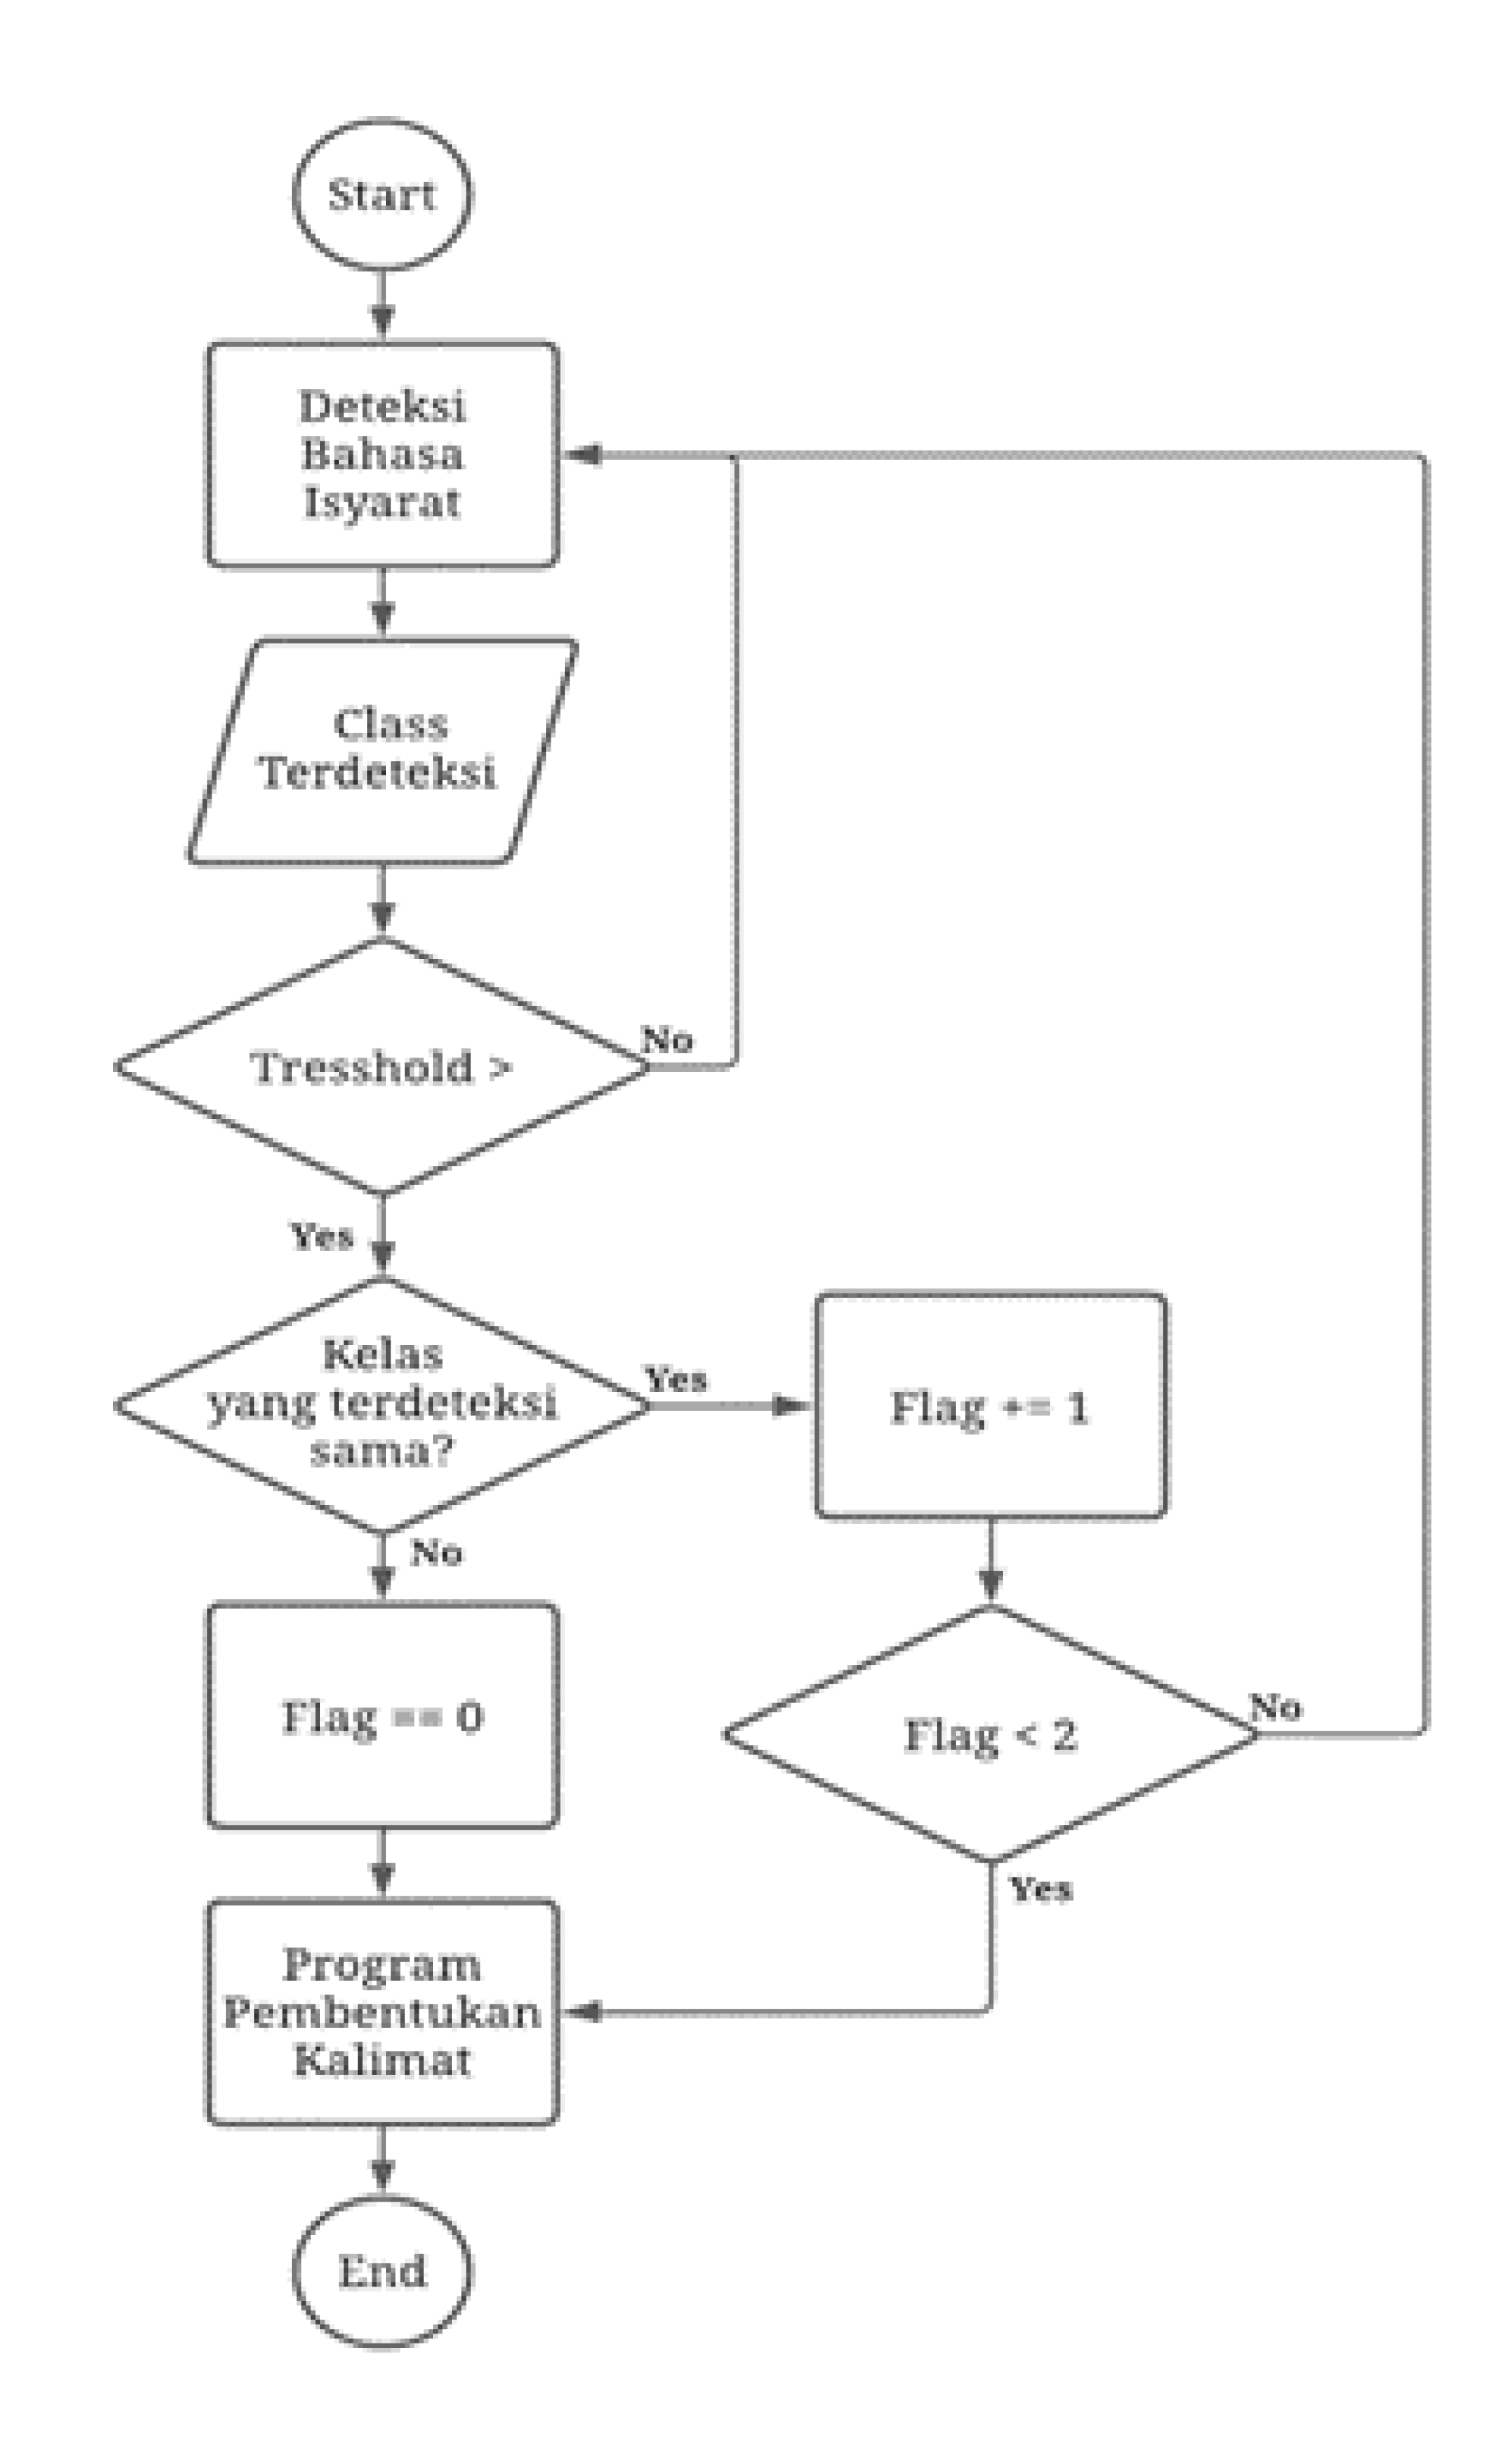
\includegraphics[scale=0.35]{gambar/bab3-flowchart-deteksi.png}

  \caption{Flowchart program deteksi bahasa isyarat}
  \label{fig:flowchartdeteksi}
\end{figure}

\begin{figure}[H]
  \centering

  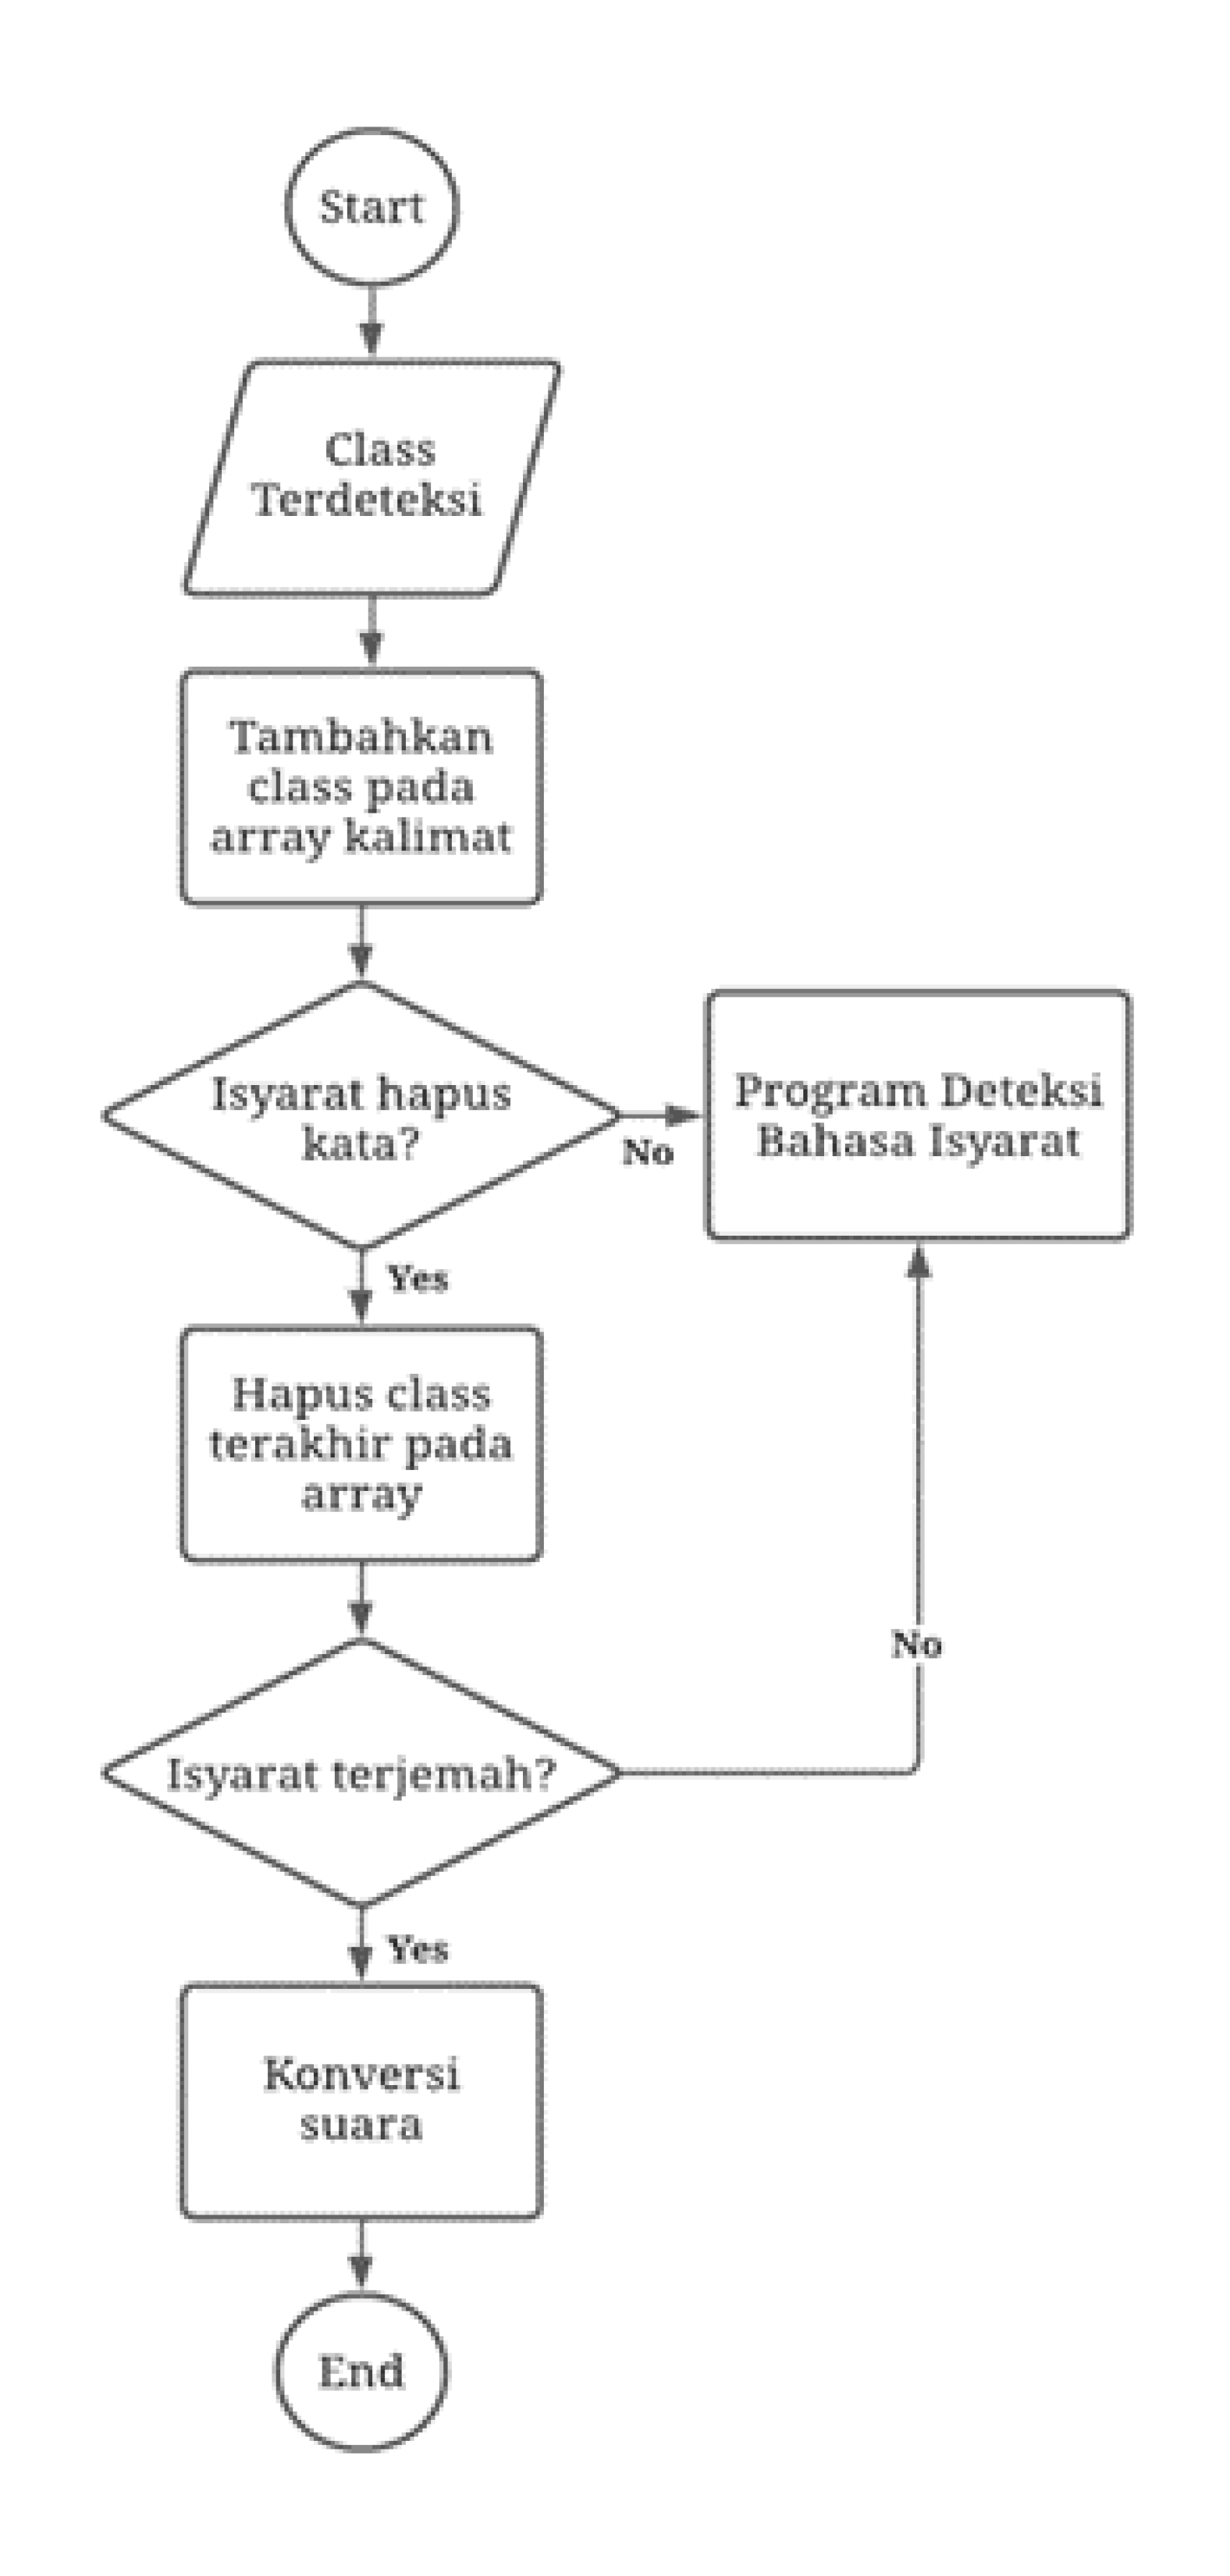
\includegraphics[scale=0.35]{gambar/bab3-flowchart-kalimat.png}

  \caption{Flowchart Program pembentukan kalimat}
  \label{fig:flowchartkalimat}
\end{figure}


\subsection{Integrasi \emph{Next Unit Computing} (NUC)}
\label{subsec:integrasiNUC}

Integrasi dengan Intel NUC dilakukan dengan mengakses website yang dibuat menggunakan \emph{framework} Streamlit penerjemah yang telah terhubung dengan server komputer menggunakan skema \emph{port forwarding}. Website akan mengakses webcam pengguna sehingga pengguna dapat melakukan gerakan isyarat yang kemudian diklasifikasikan dengan model LSTM yang telah dilatih sebelumnya secara \emph{realtime}. 
% Pada cetak biru yang tertera pada Gambar \ref{fig:cetakbiru}. \lipsum[8]

% % Contoh input gambar pada kolom.
% \begin{figure} [ht]
%   \centering
%   % Ubah sesuai dengan nama file gambar dan ukuran yang akan digunakan.
%   \includegraphics[width=0.4\textwidth]{gambar/cetakbiru.jpg}

%   % Ubah sesuai dengan keterangan gambar yang diinginkan.
%   \caption{Cetak biru roket yang akan diuji coba. \cite{cetakbiruspacex}}
%   \label{fig:cetakbiru}
% \end{figure}

% \lipsum[9-10]

% \subsection{Lorem Ipsum}
% \label{subsec:loremipsum}

% \lipsum[11]

% % Contoh pembuatan tabel.
% \begin{table}
%   \caption{Contoh tabel sederhana}
%   \label{tab:tabelsederhana}
%   \centering
%   \begin{tabular}{lll}
%     \toprule
%     Heading1 & Heading2 & Heading3 \\
%     \midrule
%     One      & Two      & Three    \\
%     Four     & Five     & Six      \\
%     \bottomrule
%   \end{tabular}
% \end{table}

% % Contoh pembuatan potongan kode.
% \begin{lstlisting}[
%   language=C++,
%   caption={Program halo dunia.},
%   label={lst:halodunia}
% ]
% #include <iostream>

% int main() {
%     std::cout << "Halo Dunia!";
%     return 0;
% }
% \end{lstlisting}

% \lipsum[12]

% % Contoh pembuatan daftar.
% \begin{enumerate}
%   \item \lipsum[13][1-4]
%   \item \lipsum[13][5-8]
%   \item \lipsum[13][9-12]
% \end{enumerate}

% \lipsum[14-15]